\paragraph{Dekoder} \mbox{} \\
En dekoder tar et n-bit signal og gir et dekodet signal på utgangen hvor bare
én pinne er høy "1".

\begin{figure}[H]
  \caption{2 til 4 linjers dekoder.}
  \centering
  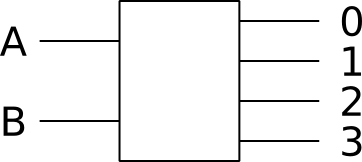
\includegraphics[width=0.5\textwidth]{./img/2to4}
\end{figure}

Sannhetstabellen viser at hver input-kombinasjon svarer til en output pin.

\begin{table}[H]
  \caption{Sannhetstabell for 2til4 dekoder.}
  \centering
  \begin{tabular}{c c | c c c c}
    A & B & 0 & 1 & 2 & 3 \\ \hline
    0 & 0 & 1 & 0 & 0 & 0 \\
    0 & 1 & 0 & 1 & 0 & 0 \\
    1 & 0 & 0 & 0 & 1 & 0 \\
    1 & 1 & 0 & 0 & 0 & 1
  \end{tabular}
\end{table}

Man kan også ha f.eks. en 4 bit dekoder med 16 output pinner.



\paragraph{Enkoder} \mbox{} \\
En enkoder fungerer motsatt av en dekoder.
Den gir n bit ut basert på $n^2$ linjer inn.
For eksempel 16 linjer inn og 4 bit ut.
\\\\
Et bruksområde kan f.eks. være en 4x4 keypad, hvor hver knapp svarer til én
av 16 pinner.
Enkoderen oversetter dette til et 4 bit signal.

\begin{figure}[H]
  \caption{Keypad enkoder.}
  \centering
  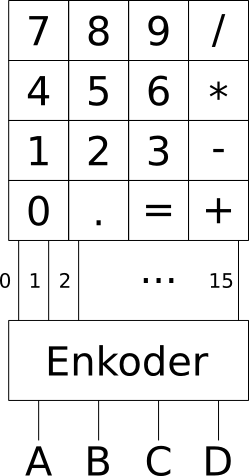
\includegraphics[width=0.5\textwidth]{./img/kp-enkoder}
\end{figure}
